%---------------------------------------------------------------------
%
%                          Capítulo 2 - Estado del arte
%
%---------------------------------------------------------------------

\chapter{Estado del arte}

\paragraph{}
En este capítulo, se pretende desglosar el estado actual así como parte de la historia que ha llevado a dicha actualidad de aquellos aspectos de la psicología (~\ref{cap1:sec:Emociones}) y la informática (~\ref{sec:iot}) que afectan de manera transversal a este trabajo. Para ello, se van a detallar los principales hallazgos tanto en psicología como en informática en lo que respecta a las emociones y su medición. Se va a comenzar con una introducción a las distintas teorías psicológicas que han pretendido acotar las emociones (~\ref{subsec:teorEmoc}), así como los métodos desarrollados para la medición de las mismas en los humanos sin mediciones fisiológicas (~\ref{subsubsec:medicionIra1}), como son los cuestionarios. Tras esto, se van a explorar los métodos para la intervención con pacientes con ira disfuncional (~\ref{subsubsec:intervencionPsico}). La parte que concierne a los aspectos psicológicos de esta sección finaliza con la fisiología de la ira (~\ref{subsubsec:fisioIra}), la revisión de los trabajos para su medición (~\ref{subsubsection:medirEmocFisio}) y la suscripción al código deontológico del Consejo General de Colegios Oficiales de Psicólogos de España (~\ref{section:codDeonto}). En lo que respecta a la parte informática, esta sección incluye un breve repaso de las aplicaciones de Internet de las Cosas (~\ref{subsec:accIntelig}) así como una comparativa entre distintas pulseras inteligentes que se barajaban para la realización de este trabajo (~\ref{subsubsec:pulserasInteligentes}) con la correspondiente explicación de la elección final de la pulsera inteligente que se ha utilizado (~\ref{subsubsec:comparativaPulseras}).

%-------------------------------------------------------------------
\section{Emociones}
\label{cap1:sec:Emociones}

\paragraph{}
Las emociones se pueden entender como una reacción subjetiva que ocurre como resultado de cambios psicológicos y fisiológicos que influyen sobre el pensamiento y la conducta \citep{psicoemocional} y que constituyen una experiencia afectiva en cierta manera agradable o desagradable \citep{montanes2005psicologia}. De manera adicional, Wundt (\citeyear{wundt1896lectures}) entendía que las emociones podían definirse según las dimensiones agrado-desagrado, tensión-relajación y excitación-calma.

\paragraph{}
En línea con las observaciones de Wundt, más adelante se simplificó dicho modelo a dos variables con las que se podían representar todas las emociones. Este es el método compuesto por el binomio valencia-activación, que presupone que todas las emociones se pueden definir mediante el nivel de agrado-desagrado (valencia) y calma-activación (activación o \textit{arousal}). El autoreporte de la emoción con este modelo se puede hacer utilizando el método \ac{SAM}, con el que el paciente determina el grado de valencia y activación en una escala de 1 a 5, 7 o 9 (el número de posibilidades la establece el profesional en cuestión) ayudado de una serie de maniquíes como los que se pueden ver en las figuras~\ref{fig:valencia-num} y~\ref{fig:activacion-num}.

\begin{figure}[h]
    \centering
    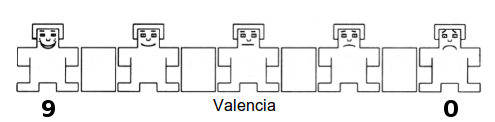
\includegraphics[scale=0.75]{Imagenes/valencia-num}
    \caption[Maniquíes para medir la valencia con el método de SAM extraídos del texto de Hernández (\citeyear{hernandez2016clasificacion}).]{Maniquíes para medir la valencia con el método de SAM (\citep{hernandez2016clasificacion}).}
    \label{fig:valencia-num}
\end{figure}

\begin{figure}[h]
    \centering
    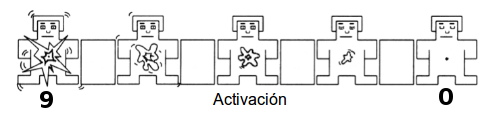
\includegraphics[scale=0.75]{Imagenes/activacion-num}
    \caption[Maniquíes para medir la activación con el método de SAM extraídos del texto de Hernández (\citeyear{hernandez2016clasificacion}).]{Maniquíes para medir la activacion con el método de SAM (\citep{hernandez2016clasificacion}).}
    \label{fig:activacion-num}
\end{figure}

Por tanto, mediante la combinación de la valencia y la activación se pueden representar todas las emociones en ejes cartesianos de dos dimensiones, tal como podemos ver en la figura~\ref{fig:valAct2}.

\begin{figure}[h]
    \centering
    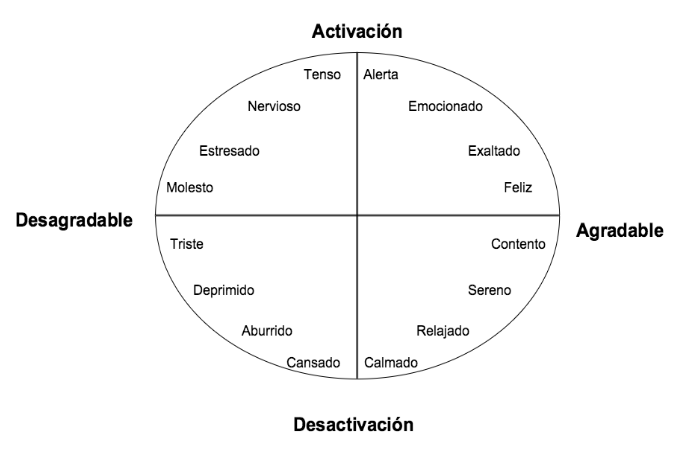
\includegraphics[width=7cm, height=7cm]{Imagenes/valAct2}
    \caption[Representación cartesiana de las emociones utilizando el binomio valencia-activación extraída del texto de Hernández (\citeyear{hernandez2016clasificacion}).]{Representación cartesiana de las emociones utilizando el binomio valencia-activación (\citep{hernandez2016clasificacion}).}
    \label{fig:valAct2}
\end{figure}

%-------------------------------------------------------------------

\subsection{Fundamentos de las emociones}
\paragraph{}
Todas las emociones tienen funciones que permiten tanto la adaptación social como el ajuste personal. Según Reeve (\citeyear{reeve1994motivacion}), la emoción tiene tres funciones principales:
\begin{itemize}
    \item Funciones adaptativas: preparan al organismo para ejecutar eficazmente la conducta exijida para las condiciones ambientales \citep{montanes2005psicologia}. Plutchik (\citeyear{plutchik1980emotion}) establece la siguiente correspondencia entre emociones y su función: miedo - protección; ira- destrucción; alegría - reproducción; tristeza - reintegración; confianza - afiliación; asco - rechazo; anticipación - exploración; sorpresa - exploración. 
    
    \item Funciones sociales: las emociones permiten que otra persona pueda anticipar el comportamiento de quien está expresando una emoción, lo que facilita las relaciones interpersonales. Así, la ira funcional sirve para que un sujeto pueda identificar que está siendo tratado injustamente y de esta manera pueda afrontar la situación con el fin de intentar enmendar dicho desajuste.
    
    \item Funciones motivacionales: la emoción energiza la conducta motivada, haciendo que esta se realice de manera más vigorosa \citep{montanes2005psicologia}. Por ejemplo, la cólera facilita las reacciones defensivas, que al haberse producido una reacción fisiológica previa, permite que las reacciones motoras puedan realizarse con mayor energía que en otro contexto en el que el cuerpo se encontrase en estado de reposo sin sentir dicha emoción.
\end{itemize}

%-------------------------------------------------------------------

\subsection{Teorías emocionales}
\label{subsec:teorEmoc}
\paragraph{}
Las principales corrientes teóricas del estudio de la emoción según Plutchick (\citeyear{plutchik1980emotion}) son:
\begin{itemize}
    \item Evolucionista: iniciada por Darwin (\citeyear{darwin1967expresion}), afirmaba que las emociones evolucionaron porque eran adaptativas y permitían a los seres humanos sobrevivir y reproducirse. Por ejemplo, el miedo impulsaba a la persona a huir o luchar.
    
    \item Psicofisiológica: iniciada por James-Lange (\citeyear{emotionJames}), establece que la fi-\\siología de las emociones precede a las mismas. Siguiendo el ejemplo anterior, este autor establece que no corremos porque tengamos miedo, sino que tenemos miedo porque corremos.
    
    \item Neurológica: iniciada por Cannon-Bard (\citeyear{emotionCannon}), rebate la teoría de James-Lange puesto que las reacciones fisiológicas asociadas a determinadas emociones puede darse sin que entre en acción la emoción correspondiente. Por ejemplo, se puede acelerar el corazón tanto al sentir miedo como al realizar actividades deportivas. Estas teorías se basan en que las emociones se producen como respuesta a un estímulo cuando el tálamo se comunica con el cerebro.
    
    \item Conductista: iniciada por James (\citeyear{james2013principles}), quien defiende en la línea de James-Lange que la reacción fisiológica es previa a la emoción. A su vez, desde esta corriente se entienden las emociones como condicionamientos aprendidos en edades tempranas.
    
    \item Teoría de la activación: iniciada por Schachter-Singer (\citeyear{schachter1962cognitive}), establece primero que la activación fisiológica precede a la emoción y que dicha activación tiene como fin preparar al individuo para situaciones de emergencia.

    \item Teoría cognitiva: iniciada por Lazarus (\citeyear{lazarus1970towards}), establece que son los procesos de valoración cognitiva los que determinan la reacción emocional, por lo que la activación fisiológica por sí sola no desencadena reacciones emocionales. Es decir, quien en última instancia determina la expresión de la emoción es la interpretación que haga el sujeto de la realidad.
\end{itemize}

%-------------------------------------------------------------------

\subsection{Emociones básicas}
\paragraph{}
Las emociones básicas serían aquellas que tendrían un carácter universal, innato y que son distintas entre ellas. A partir de sus combinaciones se podrían generar todas las demás emociones denominadas emociones secundarias o derivadas. Esta teoría es defendida por neodarwinistas como Ekman, Izard y Friesen. Izard (\citeyear{izard1992basic}) establece los siguientes requisitos para que una emoción pueda ser considerada como básica:

\begin{itemize}
    \item Tener un sustrato neural distintivo.
    \item Tener una expresión facial distintiva.
    \item Poseer sentimientos distintivos.
    \item Derivar de procesos biológicos evolutivos.
    \item Manifestar propiedades motivacionales y organizativas de funciones \\ adaptativas.
\end{itemize}

\paragraph{}
Siguiendo este criterio, Izard (\citeyear{izard1992basic}) establecía que las emociones básicas eran: placer, interés, sorpresa, tristeza, ira, asco, miedo y desprecio. Por otro lado, Ekman (\citeyear{ekman1992argument}) considera que las emociones básicas son: ira, alegría, asco, tristeza, sopresa y miedo, lista a la que más tarde añadió el desprecio. Como se puede ver, existe una importante diferencia entre las listas de emociones básicas de ambos autores. Es por ello que autores como Ortony y Turner (\citeyear{ortony1990s}) consideran que no existen emociones básicas ya que ni siquiera entre quienes defienden su existencia, señalan el mismo conjunto de emociones.

\paragraph{}
A continuación se van a describir las características principales de la ira, la emoción con la que se ha trabajado en este proyecto.

%-------------------------------------------------------------------

\subsection{La ira}

\paragraph{}
Las definiciones más extendidas de la ira la catalogan como una emoción que se presenta cuando un organismo se siente bloqueado en la consecución de una necesidad o una meta, sea esta real o fantaseada \citep{nieto2008aproximaciones}. Esta percepción puede ser respondida con un impulso de huida - miedo y ansiedad - o de ataque, en cuyo caso estaríamos hablando de la ira. Esta es una emoción social, que ha servido a lo largo de la evolución para adaptarse a cambios ambientales y activar patrones de actuación útiles para la supervivencia.

\paragraph{}
Actualmente existe un debate abierto respecto a la relación entre este ataque con la agresividad pues no todos los autores catalogan esta emoción como desencadenante de actitudes agresivas; algunos consideran a ésta como la mediadora entre la frustración y la agresión \citep{averill1983studies} mientras que otros señalan la insuficiencia de evidencia experimental para sostener este tipo de afirmaciones \citep{berkowitz1989frustration}.

\paragraph{}
El psicólogo Paul Ekman (\citeyear{ekman1997face}) considera que la expresión facial de esta emoción es universal, al igual que ocurre con el resto de emociones básicas. En la figura~\ref{fig:ekman} se puede ver la cara de una persona al experimentar la ira, cuyos rasgos físicos característicos son: el descenso y la unión de las cejas, la elevación del párpado superior e inferior, la reducción de la apertura palpebral y los labios en tensión, contraídos y apretados \citep{lairama}.


\begin{figure}[h]
    \centering
    
\includegraphics[width=5cm, height=7cm]{Imagenes/ekman-anger}
    \caption[Expresión facial de la ira según se recoge en los FACS de Ekman]{Expresión facial de la ira según se recoge en los FACS de Ekman}
    \label{fig:ekman}
\end{figure}

\paragraph{}
Existen una serie de emociones con una sintomatología similar a la ira: el miedo y la hostilidad. La ira tiende a remover obstáculos que se interponen en la consecución de la meta, mientras que la hostilidad no tiene por qué implicar el acercamiento a la misma. Sus rasgos son la irritabilidad, cinismo e interpretación negativa de las intenciones ajenas. Por su parte, el miedo tiene una sintomatología fisiológica similar a la ira, con la diferencia de que ésta es de menor intensidad en la ira y de que la ira es un sentimiento caliente y el miedo es un sentimiento frío. La diferencia del sentimiento de la ira frente al de frustración es que en la ira el obstáculo en la consecución de la meta es otra persona que además tiene cierta intencionalidad en impedir que se alcance dicho objetivo, mientras que en la frustración no existe dicha intencionalidad ni el obstáculo para alcanzar dicha meta tiene por qué ser externo. Puede ser, por ejemplo, una mala planificación temporal de cara a un examen que se conocía con suficiente antelación para haberlo podido preparar bien.

\subsubsection{Modelo transaccional de la ira}

\paragraph{}
Al categorizar la ira, el equipo de expertos de la universidad de Colorado dirigido por Deffenbacher (\citeyear{deffenbacher2000overcoming}) determinó que la respuesta de esta emoción es regulable y que sólo ocasionalmente y de manera parcial es automática e incontrolable. Para estos autores, la experiencia de la ira podía entenderse como una serie de cinco etapas que irían activándose una tras otra de manera muy rápida, lo que provocaría que la persona no fuera consciente de estar enfadada hasta experimentar la respuesta de la ira. A esta serie de cinco etapas se denomina modelo transaccional de la ira. Estas etapas son las siguientes:

\begin{itemize}
    \item Fase 1 (Estado previo de ira). La personalidad y el estado fisiológico influyen en la expresión de la ira. Por ejemplo, Aaron T. Beck (\citeyear{beck2003prisioneros}) estableció que las personas perfeccionistas, con una mayor necesidad de control, baja tolerancia a la incertidumbre o a la frustración tienden a experimentar la ira con mayor frecuencia e intensidad. A su vez, un experimento de Schieman (\citeyear{schieman2010sociological}) desveló que entre la población estadounidense los rasgos que hacen a una persona propensa a experimentar la ira era ser adultos de entre 30 y 40 años, un bajo nivel educativo, tener varios hijos y tener ingresos bajos. Respecto al estado fisiológico, si la persona tiene sueño o hambre, esto puede hacer que se reduzcan los umbrales de activación de la ira. Esta fase resume los antecedentes que pueden facilitar un episodio de ira, pero por sí sola no tiene que implicar el desencadenamiento de esta emoción.
    
    \item Fase 2 (Procesos de valoración). Como se ha comentado en la definción de la ira, en la experiencia de esta emoción se valora que en una determinada situación se está actuando de manera injusta para con el sujeto. Es en esta etapa en la que se realiza dicha valoración.
    
    \item Fase 3 (Experiencia de la ira). Una vez se ha realizado el proceso de valoración y se ha valorado afirmativamente tanto el trato injusto al sujeto como la intencionalidad en dicho trato, comienzan las reacciones fisiológicas asociadas como pensamientos que se recrean en dicha injusticia, posibles pensamientos de venganza y/o reparación así como otros pensamientos que justifican dicho sentimiento \citep{uceda2011programa}.
    
    \item Fase 4 (La expresión de la ira). En esta fase la ira se activaría de una manera adaptativa para confrontar un problema e iniciar una comunicación recíproca que permita solucionarlo o de manera desadaptativa o disfuncional, que implicaría la violencia verbal o física. 
    
    \item Fase 5 (Consecuencias de la ira). Las consecuencias de la ira dependerán fundamentalmente de si la expresión de la misma ha sido funcional o disfuncional. Si la expresión ha sido funcional, puede que se consiga solventar el problema que se percibía como injusto. En el caso de que haya sido disfuncional, la expresión puede incluso haber empeorado el problema. El motivo por el que se activaría este tipo de expresión de la ira es por dar preferencia al éxtasis del corto plazo durante la expresión frente a las consecuencias futuras en el medio o largo plazo.
\end{itemize}

\subsubsection{Causas de la ira}
%Se hace un salto de línea antes de 'concretas' porque corta mal las sílabas de esta palabra
\paragraph{}
En la mayoría de estudios sobre la ira, esta se suele acotar por el propio paciente mediante cuestionarios en los que bien se presentan situaciones con- \\ cretas que pueden provocar ira, bien se plantean afirmaciones relativas a la ira a las cuales el paciente debe responder en una escala de Likert. Un ejemplo de situación concreta que puede provocar la ira sería ``llegas tarde y el coche que tienes en frente va a 25 kilómetros por hora siendo la limitación de la carretera de 40 kilómetros por hora'', mientras que un ejemplo de afirmación relativa a la ira sería ``tengo ganas de pegarle a alguien''.

\paragraph{}
Por otro lado, en estos cuestionarios las causas que provocan la ira suelen referirse a situaciones muy específicas o demasiado difusas. Como término medio, se puede encontrar el estudio de Alcázar (\citeyear{alcazar2015que}) que versa precisamente sobre las causas que provocan la ira a los estudiantes universitarios. En este caso las fuentes que provocan ira son divididas en tres bloques:
\begin{itemize}
\item Interacción con los demás: mentiras, injusticia, impuntualidad, insultos, irresponsabilidad, traición, discusiones, prepotencia, que alguien diga lo que se tiene que hacer, pelea, hipocresía, ser ignorado, ser contradecido, ser criticado, no ser escuchado, que otra persona cambie los planes...
\item Uno mismo: que no salgan las cosas como se quería, no poder resolver algo, no poder ayudar, trabajar en algo que no se quiere, perder algo, hacer tareas, dormir poco, perder el tiempo...
\item Otros: atascos o retrasos en el transporte público, que deje de funcionar un dispositivo electrónico...
\end{itemize}

Estas situaciones como se puede ver, son bastante genéricas y permiten acotar los motivos que provocan la ira, mientras que en otros estudios que se detallarán más adelante como S.T.A.X.I. o Novaco se intenta únicamente medir la ira.

\subsubsection{Intervención psicológica de la ira disfuncional}
\label{subsubsec:intervencionPsico}

\paragraph{}
A la hora de intentar realizar una intervención efectiva en los casos en los que esté presente la ira disfuncional, es importante saber cuantificar correctamente su intensidad, duración y periodicidad. Para ello, es importante que, además de conocer la sintomatología de emociones similares tal y como se ha mencionado anteriormente, en su medición se tengan en cuenta estos tres factores:
\begin{itemize}
    \item Reactividad situacional: la ira es una emoción social que se da en ámbitos concretos y que depende de cada persona, en la que cada persona aprende los lugares en los que puede o no puede expresar dicha emoción. Es decir, la misma valoración de una situación puede provocar o no la expresión de la ira en la misma persona en función del ambiente y de las personas presentes en ese momento (una persona introvertida por ejemplo puede no sentirse cómoda expresando dicha emoción si esto supone ser el foco de atención). Por ello, para medir esta emoción es importante que la persona se sienta cómoda para poder expresarse emocionalmente como considere, sin provocar situaciones impostadas en el laboratorio en las que debido al ambiente, el sujeto pueda no expresar las emociones tal cual las sienta y de esta manera se evite obtener resultados con baja validez ecológica.
    
    \item Deseabilidad social: es una distorsión inintencionada de la realidad en la que se puede minimizar el problema a la hora de describirlo a terceros (un psicólogo, por ejemplo) por el fin inconsciente de intentar generar una buena imagen en esas personas.
    
    \item Simulación: es una distorsión intencionada de la realidad. Este factor tiene su relevancia en los casos en los que los resultados del análisis puedan tener consecuencias legales sobre el paciente, como pueda ser la presentación de un informe psicológico para un juicio.
\end{itemize}

\paragraph{}
Para evitar caer en alguno de estos errores, es recomendable utilizar enfoques multimétodo-multimomento. En este punto es precisamente en el que accesorios inteligentes no intrusivos pueden ser útiles para obtener datos fia-\\bles fuera de la consulta.


%-------------------------------------------------------------------

\subsubsection{Métodos psicológicos para la medición de la ira}
\label{subsubsec:medicionIra1}

\paragraph{}
Existen numerosas escalas de medición de emociones, en las que no todas ellas han sido validadas. Por ello, se hace especialmente relevante determinar una escala común de confiabilidad, es decir, del grado en que un instrumento de varios elementos mide consistentemente una muestra de la población \citep{celina2005aproximacion}. La escala que se suele utilizar para la medición de la ira es el alfa de Cronbach (\citeyear{cronbach1951coefficient}), que define el grado de correlación existente entre una serie de elementos y aquellos que se quiere medir. Por ejemplo, la correlación entre que el cielo esté nublado y que vaya a llover en la próxima hora es mayor que entre que el día que se quiera saber si va a llover es par o impar, que no tiene ninguna relación con aquello que se pretende inferir, por lo que el hecho de que el dato de si está el cielo nublado o no tendrá un alfa de Cronbach mayor que si el día es par a impar. De la misma manera, se pueden comparar un conjunto de preguntas, que suelen ser denominados métodos o modelos.

\paragraph{}
En el caso que nos concierne, el dato que se quiere inferir es el valor discretizado en el que se encuentra una persona en una escala de de la ira. Cuanto más elevado sea el alfa de Cronbach (en una escala de 0 a 1) para un modelo, mayor será la fiabilidad del mismo. Concretamente, la medición de la ira será desglosada en dos apartados: estado del rasgo de la ira, que evalúa los distintos componentes de la intesidad de esta emoción y su expresión verbal y física y la escala de rasgo de la ira, que mide el temperamento y la reacción de la ira en el sujeto evaluado. 

\paragraph{}
A continuación se citan algunos de los métodos utilizados en psicología para la evaluación de la ira:

\begin{itemize}
    \item S.T.A.X.I. 2 \citep{spielberger}. Es un cuestionario que cuenta con 49 sentencias que miden la experiencia, la expresión y el control de la ira. La escala empleada para responder a las cuestion es de tipo Likert, es decir, incluyen varias opciones según la conformidad con la afirmación realizada (absoluto-mucho, nunca-siempre) a sentencias como ``me siento furioso'' o ``siento que quiero romper cosas''. Estas 49 cuestiones pretenden evaluar al sujeto en los siguientes aspectos: ira en el momento en el que realiza el cuestionario, ira como un rasgo de la persona y por tanto duradero en el tiempo, expresión externa e interna de la ira, control externo e interno de la ira e índice de expresión de la ira, que correlaciona la expresión externa con la expresión interna de la ira. En cuanto a su fiabilidad, en este test obtiene un 0.89 de coeficiente de alfa de Cronbrach en la escala del estado de la ira y un 0.82 en la escala de rasgo de la ira. Este cuestionario ha sido validado para selección de personal e investigación médica \citep{de1997anger, turnage1991job}.

    \item Novaco Anger Inventory \citep{novaco2003novaco}. Es un cuestionario con escala Likert que cuenta con 25 situaciones que pueden provocar la ira en las que se pretende que el sujeto responda el grado de intensidad de la ira que estas provocarían en el sujeto. Algunas de estas situaciones que se plantean son ``alguien ha cometido un error y te culpa'', ``estás intentando discutir algo importante con un amigo o un familiar y no te está dejando la posibilidad de expresar tus sentimientos'' o ``que tu coche se quede atascado en el barro o la nieve''. Este cuestionario ha sido aplicado a adultos que habían cometido infracciones correccionales y entre población con problemas clínicos de gestión de la ira \citep{mills1998novaco, jones1999normative}. En el caso del estudio de Mills, Kroner y Forth (\citeyear{jones1999normative}), el cuestionario de Novaco clasificó correctamente a los pacientes clínicos con una precisión del 94\%. El alfa de Cronbach no se incluyó entre los resultados de validación de este cuestionario.

    \item Inventario de hostilidad de Buss y Durkee (BDHI) \citep{buss1957inventory}. Es un cuestionario de 75 elementos de verdadero o falso que pretenden cuantificar la ira y la hostilidad en sus componentes experienciales y expresivos. Algunas de las cuestiones que se plantean son ``raramente pego a alguien, aun si la persona me pega a mí primero'', ``sé que la gente tiende a hablar mal de mí a mis espaldas'' o ``cuando la gente me grita, yo le grito de vuelta''. Este cuestionario permite medir de forma válida la agresión física y verbal, la ira y la hostilidad en sujetos españoles \citep{lopezvalidacion}. Por otro lado, en un experimento realizado para medir la fiabilidad de este cuestionario, este test obtuvo un alfa de Cronbach de 0.83 \citep{grana2001tipologia}.

    \item Inventario de Pensamientos Relacionados con la Ira y la hostilidad (IPRI) \citep{sukhodolsky2001development}. Es un cuestionario de 26 elementos de tipo Likert que intenta medir la frecuencia en la que el sujeto ha tenido en las últimas semanas pensamientos automáticos asociados a la ira-hostilidad. Las cuestiones están repartidas entre estas cuatro categorías: pensamientos posteriores de ira, pensamientos de venganza, recuerdos que provoquen la ira y el entendimientos de las causas. Algunas de las cuestiones de este cuestionario son ``pienso en los motivos por los que la gente me trata mal'', ``rumio por experiencias de ira pasadas'' o ``recuerdos de molestias pequeñas me molestan durante un tiempo''. En cuanto a su fiabilidad, este cuestionario obtiene un 0.88 de coeficiente de alfa de Cronbach \citep{prieto2000modelo}.
\end{itemize}

\subsubsection{Métodos psicológicos para la intervención con pacientes con ira disfuncional}

\paragraph{}
Una vez se ha evaluado la ira en una persona, en caso de que los resultados obtenidos sean de que ésta se presenta de manera disfuncional, es importante ayudar al paciente a regular esta emoción. A continuación se describen algunas de las propuestas utilizadas para este fin:

\begin{itemize}
    \item Deffenbacher y McKay (\citeyear{deffenbacher1996expression}) proponen un método con los siguientes ejes: aumentar la conciencia del problema mediante preguntas introspectivas, interrumpir el desarrollo de la respuesta de la ira mediante autoinstrucciones, utilizar el entrenamiento por relajación mediante la visualización mental de imagenes que inciten a la calma, reestructuración cognitiva para intentar que los juicios que pueden llevar a la expresión de la ira sean menos dicotómicos y catastrofistas.

    \item Lochman y Wells (\citeyear{lochman1996social}) proponen una mayor concienciación de las seña- \\ les fisológicas asociadas a la ira, aumento de las habilidades sociales para gestionar los problemas de manera más adaptativa y la técnica de tiempo fuera (en caso de no haber conseguido evitar la aparición de la ira de manera disfuncional y ser consciente de ello, alejarse durante unos cuantos segundos de la situación hasta que la reacción fisiológica y cognitiva asociada a la emoción mermen).

    \item Novaco (\citeyear{novaco2003novaco}) propone un enfoque que tiene como ejes principales el aumento de la autoestima del sujeto, pues esto reducirá la probabilidad de que éste responda a provocaciones \citep{rosenbaum1960direct} \citep{veldman1961defensiveness} y aumento no sólo del control de la ira, sino también de la sensación de dicho control, pues de esta manera se aumenta a su vez dicho control de la ira.

    \item Beck (\citeyear{beck1998cognitive}) divide la intervención psicoterapeuta en tres fases. En la primera, denominada fase preventiva, se explica al paciente el \\ funcionamiento de la ira. La segunda, denominada fase de intervención, se centra en los procesos de valoración y en la desactivación fisiológica mediante técnicas de relajación. En la tercera, denominada fase de postvención, en aquellos casos en los que la ira no disminuye, se ahonda en el contexto en el que se da la reacción de la ira.
    
    \item Kendall y Braswell (\citeyear{braswell1985involvement}) se centran en el control de la respuesta impulsiva ante la aparición de problemas, evaluando por tanto en qué medida se preferencia el cortoplacismo a los análisis de medio y largo plazo. Las fases de este modelo son: reconocimiento y definición del problema, desarrollo de alternativas de resolución del problema, focalización de los elementos clave del problema; elección de la solución evitando el cortoplacismo y autorrefuerzo de este modelo resolutivo.
    
    \item Pérez Nieto y Magán Uceda (\citeyear{lairama}) proponen un modelo que consta de nueve etapas distribuidas en tres grandes bloques:
    
    \begin{itemize}
        \item Prevención
        \begin{enumerate}
            \item Cuidar la propia autoestima cuidando las elecciones
            \item Mantener una orientación hacia la tarea.
            \item Identificar escenarios y secuencias habituales de la ira.
        \end{enumerate}

        \item Regulación de la experiencia
        \begin{enumerate}
            \item Identificar las primeras sensaciones (fisiológicas y/o cognitivas) de la ira.        
            \item Reducción de la activación fisiológica.
            \item Revaloración de la relevancia de la situación y de los recursos de afrontamiento.
        \end{enumerate}
        \item Regulación de la expresión y de la respuesta
        \begin{enumerate}
            \item Expresión de deseos personales correctamente, pidiendo, sustituyendo el \textit{tú} por los \textit{mensajes yo}.
            \item Reforzarse por el autocontrol percibido.
            \item Recordar o comentar con otros, más tarde, la gestión que se hizo de la situación conflictiva y lo agradable del autocontrol conseguido.
        \end{enumerate}
    \end{itemize}    
    
    
\end{itemize}

\paragraph{}
Como se puede observar, la mayoría de las propuestas intentan cuantificar las emociones mediante la autoevaluación del sujeto. Según Picard (\citeyear{picard2009future}), los resultados obtenidos por este tipo de técnicas no son fiables (por los factores mencionados en la sección~\ref{subsubsec:intervencionPsico} como la deseabilidad social) pues por un lado un paciente puede no sentirse cómodo expresando dicha emoción con el profesional si no tiene suficiente cercanía, o puede suceder incluso que no entienda alguna pregunta debido a la ambigüedad de la misma. Por ejemplo, en la versión mexicana del cuestionario de S.T.A.X.I. 2, se adaptó el contenido de éste a la jerga mexicana, modificando expresiones respecto a la versión española. El problema es que en su sustitución varias de las frases que se utilizaron eran demasiado similares, por ejemplo: ``me siento enojado'', ``estoy enojado'' y ``estoy ardiendo de enojo'' \citep{oliva2010validacion}.



%-------------------------------------------------------------------

\subsection{Fisiología de las emociones}
\label{subsec:fisioEmoc}

\paragraph{}
Las emociones siempre van acompañadas de reacciones somáticas, siendo las más importantes las alteraciones de la circulación, los cambios respiratorios y las secrecciones glandulares. Los tres componentes de las respuestas emocionales son los siguientes:

\begin{itemize}
    \item Componente comportamental o conductual: incluye todos los movimientos musculares que se desencadenan tras una emoción (en el caso del miedo, la huida o el enfrentamiento, con sus correspondientes movimientos musculares).
    
    \item Componente neurovegetativo: comprende los cambios en el sistema ner-\\vioso autónomo para aportar una rápida movilización de energía que podría ser necesaria en caso de realizar movimientos enérgicos. En el caso del miedo, esto provocaría una activación de la rama simpática -para ganar tensión muscular y actividad cardíaca- y una desactivación de la rama parasimpática -para que la activación se centre en los músculos y no por ejemplo en procesos digestivos-.
    
    \item Componente hormonal: refuerzan las respuestas neurovegetativas mediante la secrección de hormonas como la adrenalina o la noradrenalina.
\end{itemize}

\paragraph{}
En las respuestas fisiológicas de las emociones, la amígdala juega un papel relevante, pues es donde se interpreta la información de las 	aferencias (señales que provienen de las neuronas sensoriales que transmiten información de lo que ocurre en distintas partes del cuerpo así como en el entorno) para redireccionar ésta a la región cerebral correspondiente que producirá la eferencia (respuestas neurológicas del sistema nervioso central tras la interpretación de las aferencias). En la tabla~\ref{tab:respEmoc}, se puede encontrar una lista de ejemplos de regiones cerebrales que reciben aferencias del núcleo central de la amígdala y las respuestas emocionales que controlan estas regiones.

\begin{table}[]
\caption{Regiones cerebrales que reciben aferencias de la amígdala y las respues-\\tas emocionales que controlan esas regiones.\citep{davis1992}}
\label{tab:respEmoc}
\begin{tabular}{|c|c|}
\hline
\textbf{Regiones cerebrales}                                                          & \textbf{\begin{tabular}[c]{@{}c@{}}Respuestas comportamentales\\ y fisiológicas\end{tabular}}                                                  \\ \hline
Hipotálamo lateral                                                                    & \begin{tabular}[c]{@{}c@{}}Activación simpática: aumento de la \\ frecuencia cardíaca y la presión arterial, \\ palidez.\end{tabular} \\ \hline
Núcleo motor dorsal del vago                                                          & \begin{tabular}[c]{@{}c@{}}Activación parasimpática: \\ úlceras, micción, defecación\end{tabular}                                           \\ \hline
Núcleo parabranquial                                                                  & Respiración agitada.                                                                                                                           \\ \hline
Área tegmental ventral                                                                & Alerta comportamental (dopamina).                                                                                                              \\ \hline
Locus coeruleus                                                                       & Aumento de la vigilancia (noradrenalina).                                                                                                      \\ \hline
\begin{tabular}[c]{@{}c@{}}Núcleo reticular de la\\ protuberancia caudal\end{tabular} & Aumento de la respuesta al sobresalto.                                                                                                         \\ \hline
Sustancia gris periacueductal                                                         & Cese de la conducta (congelación).                                                                                                             \\ \hline
\end{tabular}
\end{table}

\paragraph{}
Un elemento importante en la fisiología de las emociones es el aprendizaje de la lectura de las situaciones para poder anticiparse a situaciones que están por venir. Esto puede producirse mediante el aprendizaje de estímulos neutros a los que se le asocia una reacción emocional (es decir, el condicionamiento clásico). Si una perro antes de recibir su comida preferida escucha de manera consistente un timbre y no escucha ese mismo timbre cuando no recibe comida, acabará asociando mediante condicionamiento clásico que el estímulo neutro (el timbre) es ahora un estímulo condicionado que provocará la respuesta fisiológica condicionada equivalente a la respuesta incondicional; esto es, acabará salivando ante la expectativa de la comida al escuchar el timbre antes incluso de detectar la comida. Así, en el caso de los humanos, la mayoría de los miedos se adquieren por transmisión social, en lugar de por exposición directa al estímulo \citep{olsson2007learning}.

\paragraph{}
En lo que respecta a la parte fisiológica que no tiene proyección exterior, existe un campo de estudio llamado psicología de la salud que vincula las emociones con la salud entendida en toda su extensión. Así, las emociones positivas afectan de manera positiva a la salud, sucediendo lo inverso con las emociones negativas, puesto que favorecen la aparición de ciertas enfermedades al hacer más vulnerable al sistema inmunológico \citep{moure2011}. Un estudio de 1999 ya planteaba que las personas que experimentan ansiedad crónica, prolongados periodos de tristeza y pesimismo u hostilidad, tenían el doble de riesgo de contraer enfermedades como el asma, la artritis o los dolores de cabeza \citep{lopez1999}. En el caso de la ansiedad, esta puede complicar una operación médica, puesto que la reacción fisiológica que provoca es la dilatación de las venas provocando por tanto sangrados más abundantes \citep{moure2011}. En cuanto a las emociones positivas, la risa disminuye la concentración del cortisol, que es una de las hormonas directamente vinculadas al estrés, lo que potencia la actividad de los linfocitos, responsables de una correcta respuesta inmunológica \citep{berk2008cortisol}.

\paragraph{}
Todos estos parámetros se miden tras la normalización de los mismos en función del sujeto en cuestión. Una técnica habitual es establecer primeramente el valor de las variables que se quieren medir en un estado de reposo para luego compararlo con los valores a la hora de someter al sujeto a estímulos. De la misma manera, además de analizar la variación de las distintas variables fisiológicas que se quieran medir al ser expuestos a estímulos, algunos estudios ponen el foco no sólo en la tendencia sino también en la diferencia de las magnitudes entre distintos sujetos, obteniendo conclusiones como que las personas con alta ira-hostilidad tienen mayor frecuencia cardiaca en todas las fases de un experimento en el que se les inducen dichas emociones \citep{breva2000ira}.

%-------------------------------------------------------------------

\subsubsection{Fisiología de la ira}
\label{subsubsec:fisioIra}

\paragraph{}
La ira es un factor a considerar en rehabilitaciones de algunos problemas neuropsicológicos. Según un estudio publicado en \textit{Psycologycal Bulletin} \citep{millar1996meta}, la ira disfuncional llega incluso a aumentar en un 8\% el riesgo de mortalidad cardiovascular. Teniendo en cuenta los problemas de indentificación de la ira de pacientes con problemas psicológicos como aquellos con TEA, la identificación externa de la ira disfuncional mediante la medición fisiológica del paciente, puede servir para mejorar su salud mediante la adquisión de mayor conocimiento sobre dicha emoción que le puedan servir para una canalización de la misma que no afecte a su salud.

\paragraph{}
Combinando las conclusiones de Stemmer (\citeyear{stemmler2010somatovisceral}) y Spielberger y Krasner (\citeyear{spielberger1988}), se obtiene la siguiente caracterización de la respuesta fisiológica de la ira:
\begin{itemize}
    \item Aumento de la presión arterial sistólica y diastólica (\ac{BVP}, \ac{PPG}, \ac{PCG}).
    \item Aumento de la tasa cardíaca (\ac{HR}, \ac{ECG}, \ac{ICG}).
    \item Aumento de la conductividad de la piel (\ac{EDA}).
    \item Aumento de la tensión muscular (\ac{EMG}).
    \item Aumento de la temperatura periférica facial.
    \item Aumento de la tasa respiratoria (\ac{RESP}).
    \item Enrojecimiento de la piel (\ac{SKT}).
    \item Temblores.
    \item Sensación de desmayo.
    \item Sudores fríos.
    \item Sudor de manos.
    \item Dolor de estómago.
    \item Náuseas.
\end{itemize}

\paragraph{}
Estos cambios fisiológicos son en cierto grado distintos para cada persona y se establecen como cambios respecto a su estado de reposo. Este estado de reposo en casos en los que se miden las constantes fisiológicas exclusivamente en el laboratorio se realizan solicitando al paciente que se relaje durante unos quince minutos, momento en el que se extraen sus valores mínimos, mientras que en casos en los que estas mediciones se realizan mediante accesorios inteligentes que el paciente lleva puestos durante su día cotidiano, estos valores de reposo se obtienen durante el periodo en el que el paciente duerme. El primero de estos métodos puede ser bastante problemático e inducir a errores de medición si dichos pacientes no consiguen relajarse durante ese periodo de tiempo y los investigadores no se percatan de esto, mientras que con el segundo método las constantes fisiológicas obtenidas que establecen que dicho paciente se encuentra en reposo son bastante más fiables \citep{peter2005wearable}.

\paragraph{}
Por último, un estudio de la Universidad de Murcia \citep{breva2000ira} pone de manifiesto la correlación entre los latidos por minuto del sujeto tanto en estado de reposo como en situaciones de estrés y los resultados obtenidos en tests de medición de la ira. En el experimento realizado, se utilizó como test de medición el inventario de Hostilidad de Cook y Medley (\citeyear{cook1954proposed}), dividiendo a los sujetos según los resultados obtenidos entre los grupos de baja ira-hostilidad y alta ira-hostilidad. Como se puede ver en la tabla~\ref{tab:frecCard}, la diferencia de la tasa de latidos por minuto entre estos dos grupos independientemente de la fase del experimento es de en torno a 5 latidos por minuto

\begin{table}[h]
\centering
\caption{Valores medios y desviaciones típicas de la frecuencia cardíaca en las tres fases del experimento de la universidad de Murcia}
\label{tab:frecCard}
\begin{tabular}{c|c|c|c|}
\cline{2-4}
                                                   & \textbf{Habituación} & \textbf{Tarea} & \textbf{Recuperación} \\ \hline
\multicolumn{1}{|c|}{\textbf{Baja ira-hostilidad}} & 92.27 (16.61)        & 92.43 (15.13)  & 86.35 (13.04)         \\ \hline
\multicolumn{1}{|c|}{\textbf{Alta ira-hostilidad}} & 96.95 (16.05)        & 97.02 (14.63)  & 91.48 (13.20)         \\ \hline
\end{tabular}
\end{table}

%-------------------------------------------------------------------

\subsubsection{Soluciones para medir emociones a partir de señales fisiológicas}
\label{subsubsection:medirEmocFisio}

\paragraph{}
En esta sección se esquematizan diversas soluciones tecnológicas que miden las emociones en función de datos fisiológicos. No todas las soluciones utilizan acesorios inteligentes, es más, algunas de ellas han sido sensorizadas en el laboratorio. En algunos casos los datos se han procesado posteriormente con varios clasificadores, en cuyo caso se ha incluído el clasificador que haya obtenido mayor fiabilidad. Las soluciones cuya fiabilidad está representada mediante varios números son aquellas en las que se ha medido las emociones usando la valencia y la activación, representando por tanto la fiabilidad de los resultados para cada uno de estos dos indicadores. Finalmente, es necesario indicar que la mayor parte de las referencias incluidas en esta sección son un subconjunto de dos tablas del trabajo de López Hernández (\citeyear{hernandez2016clasificacion}), si bien ha sido necesario consultar el contenido de los artículos citados puesto que en algunas ocasiones las tablas de López Hernández (\citeyear{hernandez2016clasificacion}) no incluían todos los datos que se estaban buscando, los datos eran confusos o directamente no coincidían con el artículo que se estaba citando.

\begin{enumerate}
    \item Changchun Liu (\citeyear{liu2008physiology}).
    \begin{itemize}
        \item Dispositivo: Biopac MP150.
        \item Respuestas fisiológicas analizadas: \ac{ECG}, \ac{EDA}, \ac{EMG}, \ac{ICG}, \ac{PCG}, \ac{PPG}, \ac{SKT}. 
        \item Emociones: inmersión, gusto y ansiedad.
        \item Participantes del experimento: 6 participantes de entre 13 a 16 años, 5 de ellos hombres y 1 mujer en la que 2 de ellos tenían TEA, 1 sufría Asperger y los otros 3 sufrían \ac{PDD-NOS}.
        \item Descripción de la/s tarea/s realizada/s durante el experimento: juego en el ordenador al videojuego Pong\citep{lowood2009videogames} en 3 sesiones de 1 hora distribuídas entre 3 días distintos y resolución de anagramas en 3 sesiones de 1 hora distribuídas entre 3 días distintos entre sí y entre los días de las sesiones de Pong.
        \item Clasificador: \ac{SVM}.
        \item Precisión: 83\%.
    \end{itemize}

    \item Kyung Kim (\citeyear{kim2004emotion}).
    \begin{itemize}
        \item Dispositivo: Biopac MP100.
        \item Respuestas fisiológicas analizadas: ECG, EDA, SKT.
        \item Emociones: sorpresa, estrés, enfado y tristeza.
        \item Participantes del experimento: aproximadamente 191 sujetos (no se especifica la cifra exacta) de entre 5 y 8 años.
        \item Descripción de la/s tarea/s realizada/s durante el experimento: para la inducción de la sorpresa, se subió repentinamente el volúmen de la música de fondo o se reprodución el sonido de un vaso roto; para inducir el estrés se les sometía a la realización de una tarea imposible en un periodo de tiempo corto, no se les dejaba concentrarse en la misión, la iluminación parpadeaba o se les comparaba de manera desfavorable respecto al resto de sujetos; para inducir el enfado se les enseñaba un juguete con una apariencia desagradable o se cambiaba la iluminación al color rojo; oara inducir la tristeza se les contaba una historia que evocaba simpatía con una voz lagrimosa, se ponía música de fondo triste o se cambiaba la iluminación al color azul.
        \item Clasificador: SVM.
        \item Precisión: 62\%.
    \end{itemize}

    \item Eun-Hye Jang (\citeyear{jang2013classification}).
    \begin{itemize}
        \item Dispositivo: Biopac MP150.
        \item Respuestas fisiológicas analizadas: ECG, EDA, PPG, SKT.
        \item Emociones: aburrimiento, dolor y sorpresa.
        \item Participantes del experimento: 217 estudiantes de colegios universitarios de entre 20 y 24 años compuestos por 97 hombres y 120 mujeres.
        \item Descripción de la/s tarea/s realizada/s durante el experimento: el dolor fue inducido mediante el uso de un esfigmomamómetro; el aburrimiento fue inducido mediante la escucha repetida de los números enteros comprendidos entre uno y diez y la sopresa fue inducida mediante la reproducción de sonidos de relámpagos o de vasos rompiéndose durante la realización de tareas que requerían concentración.
        \item Clasificador: \ac{LDA}.
        \item Precisión: 75\%.
    \end{itemize}

    \item Pramila Rani (\citeyear{rani2006empirical}).
    \begin{itemize}
        \item Dispositivo: Biopac (versión no especificada).
        \item Respuestas fisiológicas analizadas: BVP, ECG, EDA, EMG, ICG, PPG, SKT.
        \item Emociones: inmersión, ansiedad, aburrimiento, frustración e ira.
        \item Participantes del experimento: 15 personas entre 21 y 57 años compuesto por 7 hombres y 8 mujeres.
        \item Descripción de la/s tarea/s realizada/s durante el experimento: seis sesiones distribuidas en seis días diferentes del mismo mes, teniendo una duración de una hora por sesión. En estas sesiones, se monitorizaba con un Biopac al usuario durante los 10 primeros minutos para medir la variabilidad fisiológica del usuario de ese día. Tras esto, se sometía al paciente a series de ejercicios de resolución de anagramas de 3 minutos, un cuestionario posterior sobre sus percepciones emocionales durante el desarrollo de la tarea. Estas series también incluían jugar al videojuego Pong durante 4 minutos seguido de un cuestionario de las mismas características.
        \item Clasificador: SVM.
        \item Precisión: 86\%.
    \end{itemize}

    \item Andreas Haag (\citeyear{haag2004emotion}).
    \begin{itemize}
        \item Dispositivo: Procomp+.
        \item Respuestas fisiológicas analizadas: BVP, ECG, EDA, EMG, RESP, SKT.
        \item Emociones: todas, a través de la medición de la activación y la valencia.
        \item Participantes del experimento: no especificado.        
        \item Descripción de la/s tarea/s realizada/s durante el experimento: se inducieron las emociones mediante la muestra de imágenes del catálogo de \ac{IAPS}.
        \item Clasificador: \ac{RNA}.
        \item Precisión: 90-96\%.
    \end{itemize}

    \item Jerritta Selvaraj (\citeyear{selvaraj2013classification}).
    \begin{itemize}
        \item Dispositivo: Power Lab data Acquisition System.
        \item Respuestas fisiológicas analizadas: BVP, ECG, EMG, RESP, SKT.
        \item Emociones: neutral, feliz, triste, miedo, sorpresa, asco.
        \item Participantes del experimento: 60 sujetos de entre 9 a 68 años compuesto por 30 mujeres y 30 hombres.
        \item Descripción de la/s tarea/s realizada/s durante el experimento: visionado de vídeos con contenido emocional.
        \item Clasificador: \ac{FKNN}.
        \item Precisión: 76\%.
    \end{itemize}

    \item Pedro Nogueira (\citeyear{nogueira2013hybrid}).
    \begin{itemize}
        \item Dispositivo: NeXus-10 MKII.
        \item Respuestas fisiológicas analizadas: EDA, EMG, HR.
        \item Emociones: todas, a través de la medición de la activación y la valencia.
        \item Participantes del experimento: 22 participantes de entre 22 a 31 años.
        \item Descripción de la/s tarea/s realizada/s durante el experimento: sesiones de 2 horas en las que se inducían emociones a los participantes en tres fases bien diferenciadas: en la primera, se reproducía música clásica, en la segunda, la persona jugaba a un juego de miedo llamado Slenderman y en la tercera, el participante era expuesto a imágenes de la IAPS. En la primera y la segunda fase, se pedía al participante que autoreportasen su arousal y valencia en una escala de Likert de -5 a 5 en intervalos de 0.5. En el caso de Slenderman, estos valores se obtuvieron de la grabación y posterior análisis del paciente así como de una entrevista personal una vez finalizada la partida del juego.
        \item Clasificador: modelos de regresión y RF.
        \item Precisión: 91\% - 96\%.
    \end{itemize}

    \item Choubeila Maaoui (\citeyear{maaoui2010emotion}).
    \begin{itemize}
        \item Dispositivo: Procomp Infinity.
        \item Respuestas fisiológicas analizadas: BVP, EDA, EMG, RESP, SKT.
        \item Emociones: diversión, desprecio, disgusto, miedo, neutral y tristeza.
        \item Participantes del experimento: 10 sujetos de entre 23 y 30 años compuestos por 7 hombres y 3 mujeres.
        \item Descripción de la/s tarea/s realizada/s durante el experimento:  se inducieron las emociones mediante la muestra de imágenes del catálogo de IAPS.
        \item Clasificador: SVM.
        \item Precisión: 95\%.
    \end{itemize}

    \item Eun-Hye Jang (\citeyear{jang2015analysis}).
    \begin{itemize}
        \item Dispositivo: Biopac MP150.
        \item Respuestas fisiológicas analizadas: EDA, ECG, PPG, SKT.
        \item Emociones: aburrimiento, dolor y sorpresa.
        \item Participantes del experimento: 217 sujetos de en torno a 20 años compuestos por 97 hombres y 120 mujeres.
        \item Descripción de la/s tarea/s realizada/s durante el experimento: el dolor fue inducido mediante el uso de un esfigmomamómetro; el aburrimiento fue inducido mediante la escucha repetida de los números enteros comprendidos entre uno y diez y la sopresa fue inducida mediante la reproducción de sonidos de relámpagos o de vasos rompiéndose durante la realización de tareas que requerían concentración.
        \item Clasificador: \ac{DFA}.
        \item Precisión: 85\%.
    \end{itemize}

    \item Christine Lisetti (\citeyear{lisetti2004using}).
    \begin{itemize}
        \item Dispositivo: BodyMedia SenseWear Armband.
        \item Respuestas fisiológicas analizadas: ECG, EDA, SKT.
        \item Emociones: tristeza, miedo, sorpresa, frustración y diversión.
        \item Participantes del experimento: 14 sujetos de entre 18 a 35 años compuestos por 7 hombres y 7 mujeres.
        \item Descripción de la/s tarea/s realizada/s durante el experimento: visionado de vídeos con contenido emocional.
        \item Clasificador: \ac{MBP}.
        \item Precisión: 84\%.
    \end{itemize}

    \item Thomas Friedrichs (\citeyear{friedrichs2015simple}).
    \begin{itemize}
        \item Dispositivo: Olimex Shield-EKC-EMG.
        \item Respuestas fisiológicas analizadas: ECG, EDA.
        \item Emociones: valencia para emociones englobadas como positivas o negativas.
        \item Participantes del experimento: 47 estudiantes universitarios compuestos por 26 hombres y 21 mujeres.
        \item Descripción de la/s tarea/s realizada/s durante el experimento: juego en el ordenador al videojuego Dino Run.
        \item Clasificador: SVM.
        \item Precisión: 70\%.
    \end{itemize}

    \item Gaetano Valenza (\citeyear{valenza2014revealing}).
    \begin{itemize}
        \item Dispositivo: ECG100C.
        \item Respuestas fisiológicas analizadas: ECG.
        \item Emociones: activación y valencia.
        \item Participantes del experimento: 30 sujetos de entre 21 y 24 años.
        \item Descripción de la/s tarea/s realizada/s durante el experimento: se inducieron las emociones mediante la muestra de imágenes del catálogo de IAPS.       
        \item Clasificador: SVM.
        \item Precisión: 80\%.
    \end{itemize}

    \item Fatma Nasoz (\citeyear{nasoz2004emotion}).
    \begin{itemize}
        \item Dispositivo: BodyMedia SenseWear Armband.
        \item Respuestas fisiológicas analizadas: ECG, EDA, SKT.
        \item Emociones: tristeza, ira, miedo, sorpresa, frustración y diversión.
        \item Participantes del experimento: 14 personas de entre 18 a 35 años compuestos por 7 hombres y 7 mujeres.
        \item Descripción de la/s tarea/s realizada/s durante el experimento: todos los sujetos son sometidos a la visualización de 14 vídeos extraídos de películas. De estos, 4 pretendían provocar ira, 4 diversión, 1 disgusto, 5 miedo y 4 sorpresa. Entre cada visualización de los vídeos, debían rellenar un cuestionario indicando qué emoción habían sentido. Estos resultados son luego cruzados con los obtenidos mediante el dispositivo de BodyMeadia.
        \item Clasificador: \ac{MBA}.
        \item Precisión: 84\%.
    \end{itemize}
    
    \item Guillaume Chanel (\citeyear{chanel2011emotion}).
    \begin{itemize}
        \item Dispositivo: Biosemi Active 2.
        \item Respuestas fisiológicas analizadas: BVP, EDA, RESP, SKT.
        \item Emociones: aburrimiento, compromiso (con un juego), ansiedad.
        \item Participantes del experimento: 20 sujetos con una edad media de 27 años, compuestos por 13 hombres y 7 mujeres.
        \item Descripción de la/s tarea/s realizada/s durante el experimento: los participantes tenían que jugar al Tetris en distintos niveles de dificultad en sesiones de 5 minutos, con un descanso de 90 segundos entre las sesiones para que las constantes fisiológicas volviesen al estado de reposo, momento en el que se les pedía que reportasen cómo se habían sentido cuando estaban jugando al videojuego.
        \item Clasificador: \ac{QDA} y \ac{SFFS}.
        \item Precisión: 59\%.
    \end{itemize}

    \item Luis Hernández (\citeyear{hernandez2016clasificacion}).
    \begin{itemize}
        \item Dispositivo: Empática E4.
        \item Respuestas fisiológicas analizadas: BVP, EDA, HR, SKT.
        \item Emociones: valencia y excitación.
        \item Participantes del experimento: 8 sujetos de entre 24 y 30 años compuestos por 5 hombres y 3 mujeres.
        \item Descripción de la/s tarea/s realizada/s durante el experimento: juego en una tableta electrónica al videojuego Dizzy Route.
        \item Clasificador: SVM y QDA.
        \item Precisión: 77-79\%.
    \end{itemize}

\end{enumerate}

%subsection Conclusiones

\paragraph{}
Tras analizar las soluciones presentadas, se puede ver que los dispositivos más usados son los de Biopac en distintas versiones. Biopac es una empresa especializada en la sensorización fisiológica con un amplio catálogo de productos que pueden ser combinados entre sí. Todos ellos cuentan con bastante documentación del fabricante, aunque tiene la contrapartida de no tener habilita-\\do un foro que permita la comunicación abierta entre la comunidad y los fabricantes, facilitando esto el aprendizaje colectivo. Por otro lado, un punto a considerar de estas soluciones es que muchas de ellas son de un precio superior a los 500 dólares, que es un precio muy superior a los 70-150€ que pueden costar algunas pulseras inteligentes con sensores biométricos. Además en muchos casos el único dispositivo adicional que requieren las pulseras inteligentes son un teléfono móvil con conexión a Internet para hacer de \textit{gateway}, lo que hace que las pulseras inteligentes sean una solución más accesible y asequible que las soluciones que propone Biopac. Las dos respuestas fisiológicas que aparecen con mayor frencuencia son ECG y EDA, que además, tal y como se comentó en la sección~\ref{subsec:fisioEmoc} coinciden con dos respuestas fisiológicas que se pueden utilizar para detectar la ira. Por otro lado, se puede ver que la gran mayoría de constantes fisiológicas coinciden entre los distintos experimentos, a excepción de alguna como ICG y PPG. En cuanto a la medición de las emociones, todas ellas miden al menos tres de ellas, existiendo una preponderancia de soluciones que miden todas ellas a través de la valencia y la excitación. Con el fin de generarles estas emociones, los participantes han realizado tareas bastante diversas con el factor común entre ellas de que ninguno de estos experimentos ha incluído estudios de campo o ejercicio físico. Los dos enfoques mayoritarios han consistido en la inducción de emociones mediante distintos medios audiovisuales (por ejemplo, con música de distintos tipos o vídeos) o mediante la realización de tareas como puede ser jugar a videojuegos o resolver tareas con las que se pretenda generar estrés en el paciente.

\paragraph{}
Entre los clasificadores utilizados, se puede observar un claro predominio de SVM, bien como clasificador único, bien como parte de una cadena de clasificadores, como puede ser QDA o RNA. La precisión que se obtiene con este clasificador varía entre las soluciones entre el 62 y el 95\%. En la comparativa entre las soluciones que intentan medir un conjunto concreto de emociones frente a aquellas soluciones que pretenden medir todas ellas mediante la valencia, se puede observar que no existen diferencias significativas en las precisiones alcanzadas. Por otro lado, la precisión conseguida en cada una de estas pruebas debe ser analizada con cautela, pues entre ellas hay una gran variación entre las tareas a realizar durante el experimento, la medición objetivo y los métodos de evaluación, por lo que sería incorrecto evaluar de manera aislada cada una de las variables de los distintos experimentos, al no permanecer constantes el resto de ellas. Por ejemplo, la precisión alcanzada en cualquiera de estos experimentos puede variar entre aquellos que intentan inducir una emoción al paciente y contrastan esta (que se establece como variable fija) con la emoción detectada en el experimento con aquellos casos que esta evaluación se realiza respecto a una escala de Likert rellenada por el paciente, pues no existe una correspondencia perfecta entre la autopercepción de una emoción pasada que aquella que se experimentó en aquel momento.

%-------------------------------------------------------------------

\section{Internet de las cosas}
\label{sec:iot}
\paragraph{}
El concepto de Internet de las cosas (IOT) se puede definir como una infraestructura global que permite servicios avanzados a partir de una interconexión física y virtual de las cosas basado en tecnologías de información interoperable \citep{itu2012new}. Es importante recalcar el plural en lo que respecta a la tecnología: IOT no hace referencia a una tecnología concreta, sino más bien a un conglomerado de ellas que se presentan con una estructura que en su conjunto las define como tal.

\paragraph{}
Las diferentes arquitecturas de IOT que han propuesto los desarrolladores son las siguientes \citep{said2013towards, stojmenovic2014fog}:
\begin{itemize}
    \item Arquitectura de tres capas: es la arquitectura más básica. Se compone de las siguientes capas:
    \begin{itemize}
        \item Capa de percepción: es la capa física en la que se encuentran los sensores y actuadores que interactúan con el mundo físico.
        \item Capa de comunicación: sirve para comunicar los distintos dispositivos de la capa de percepción entre sí y con la nube, en la que se pueden realizar cómputos más pesados y almacenar información de manera persistente.
        \item Capa de aplicación: es la responsable de aportar al usuario servicios específicos.
    \end{itemize}
    \item Arquitectura de cinco capas: es la arquitectura que deriva de la anterior. Se sustituye la capa de comunicación por las siguientes capas:
    \begin{itemize}
        \item Capa de transporte: tranfiere información entre la capa de percepción y la capa de procesado utilizando protocolos inalámbricos como 4G, RFID o NFC.
        \item Capa de procesado o de middleware: analiza y almacena los datos provinientes de la capa de transporte.
        \item Capa de negocio: gestiona el sistema IOT al completo, incluyendo las aplicaciones y la privacidad de los usuarios.
    \end{itemize}
    \item Arquitectura cloudcéntrica: como su nombre indica, está centrada en la nube. De esta manera, es en la nube donde se almacena la información persistente y los nodos se comunican con la misma cuando necesitan realizar cómputos pesados. Su principal ventaja es su escalabilidad.
    \item Arquitectura de niebla: pone el énfasis en el nodo, aumentando el cómputo de los mismos respecto a la arquitectura cloudcéntrica, requiriendo por tanto de un hardware con mayores prestaciones y un mayor consumo de electricidad en los nodos. Esta arquitectura añade cuatro nuevas capas entre la capa física y la capa de transporte:
    \begin{itemize}
        \item Capa de seguridad: se encarga de los protocolos criptográficos de comunicación, que debido a la capacidad de cómputo de los nodos, deben de requerir de poca potencia de cómputo.
        \item Capa de almacenamiento temporal: permite el almacenamiento temporal en los nodos.
        \item Capa de preprocesado: realiza el filtrado y las analíticas de los datos sensorizados.
        \item Capa de monitorización: monitoriza el consumo energético y los recursos.
    \end{itemize}
    \item IOT social: en esta arquitectura los dispositivos se comunican entre sí teniendo en cuenta el distinto grado de validez que cada elemento pondera al resto de elementos. Por ejemplo, en una instalación agrointeligente, se pueden instalar una serie de dispositivos IOT con mayor grado de precisión que los dispositivos aledaños, al que se le daría un mayor puntuación en esta arquitectura en caso de discordancia severa entre las mediciones de ambos sensores.
\end{itemize}

Algunas de las soluciones para los que se utiliza y se puede utilizar IOT son las siguientes \citep{atzori2010internet}:
\begin{itemize}
    \item Transportes, como el transporte mediante drones autodirigidos \citep{amazon}, conducción asistida o monitorización de parámetros ambientales como la contaminación.
    \item Entornos inteligentes, que incluye el establecimiento de la temperatura óptima de una sala según el número de ocupantes, virtualización de imágenes que permitan amenizar la visita a un museo o entrenadores personales que interactúen directamente con las máquinas del gimnasio estableciendo los parámetros personalizados del ejercicio.
    \item En el dominio social, podría servir para reforzar la memoria del usuario en función de las emociones que experimente (por ejemplo, para recordar aquella información en la que el usuario estaba especialmente alegre o distraído) \citep{picard1997affective} o incluyendo agendas que automáticamente calendaricen nuevos eventos a medida que se vaya conociendo su fecha futura.
\end{itemize}

Algunos de los principales dilemas a los que hay que buscar solución en IOT son los siguientes:
\begin{itemize}
    \item Estandarización: todavía no se ha conseguido estandarizar los protocolos de comunicación utilizados, lo que en algunos casos dificulta la integración de hardware de distintos proveedores que puede que hayan diseñado su correspondiente middleware orientándolo a distintos protocolos.
    
    \item Direccionamiento de los nodos: el protocolo de direccionamiento IPv4 que frecuentemente se usa a nivel de usuario deja de ser válido para soluciones IOT debido a la escalabilidad. Es decir, este protocolo no contiene todas las direcciones necesarias para identificar a los nodos en la red. Una de las opciones que se proponen es utilizar IPv6, que en lugar de contar con direcciones de 4 bytes, cuenta con direcciones de 16 bytes.
    
    \item Seguridad, privacidad y propiedad de los datos: las soluciones IOT por lo general son altamente vulnerables, dado que la baja potencia computacional de los nodos no permite la utilización de métodos criptográficos computacionalmente costosos. En lo que respecta a los ataques físicos, en casos en los que estos deben estar al aire libre como es el caso de los detectores de contaminación, estos tienen el riesgo de manipulación física, que además si dicho sensor recoge datos de manera continua, supone que el ataque físico no puede restringirse horariamente. Respecto a la privacidad y la propiedad de los datos, es importante ir más allá de la visión de los ataques cibernéticos a la tecnología y señalar el uso que puede dar la empresa en caso de ser propietaria de los datos que se almacenan en la nube. Algunas soluciones en cuanto a la privacidad de los usuarios son la anonimización de los mismos antes de ser guardados en la nube (por ejemplo, un sensor que utilice una cámara puede distorsionar la imagen antes de guardarla en la nube). En algunos casos, puede llegar incluso a que la propia instalación tenga servicios adicionales cuyo único fin sea la recolección de dichos datos por parte de la empresa propietaria de los mismos \citep{roomba} que pueda llegar a vender a otras empresas \citep{venkataramanan2014my}.
\end{itemize}

%-------------------------------------------------------------------

\subsection{Acesorios inteligentes}
\label{subsec:accIntelig}
\paragraph{}
Los acesorios inteligentes (también denominados \textit{wearables}) son objetos que se usan cotidianamente que han sido informatizados para, en muchos casos, convertirse en dispositivos IOT. Los más comunes son las pulseras y relojes que ofrecen al usuario información sobre su salud en función de determinados parámetros que la propia pulsera/reloj mide, o simplemente permitir otro modo de interacción tecnológica con acceso a internet.

\paragraph{}
Entre la amplia variedad de accesorios inteligentes, mientras en el ámbito laboral es bastante frecuente la presencia de aquellos que no requieren de sensores biométricos y tienen la función de registro de información (por ejemplo, para facilitar la firma de un cliente que acaba de comprar un producto), en el ámbito doméstico existe una preponderancia de accesorios inteligentes enfocados a la salud. En  el caso de estos últimos, es más probable que lo compren personas que ya siguen hábitos saludables y que quieren cuantificar sus progresos \citep{bhas2013smart}. A su vez, un estudio realizado en Inglaterra mostraba que un tercio de los practicantes de medicina reportaban que los pacientes acudían a su consulta con sugerencias basadas en búsquedas en internet \citep{cello}. En lo que respecta a los acesorios inteligentes, un 15\% de los consumidores de Estados Unidos actualmente hace uso de ellos \citep{piwek2016rise}. Por tanto, es importante tener en cuenta que actualmente hay un apoyo importante por parte del usuario en medios tecnológicos a la hora de cuidar de su salud.

\paragraph{}
Sin embargo, a largo plazo los accesorios inteligentes dejan de ser utilizados por sus usuarios. Un estudio obtenía que el 32\% de los usuarios dejaban de utilizar los acesorios inteligentes después de 6 meses, y el 50\% después de un año \citep{ledger2014inside}. Esto se puede deber a que dicha compra se produzca por fetiche y dichos accesorios inteligentes sean una solución en búsqueda de un problema \citep{piwek2016rise}. A su vez, la personalidad del usuario y su percepción de la utilidad del accesorio inteligente influye notablemente en el alargamiento o acortamiento del uso que haga de estos acesorios inteligentes \citep{ehrenberg2008personality}.

\paragraph{}
Por otro lado, como se ha comentado anteriormente existe una relación entre la salud y las reacciones fisiológicas que además pueden ser medidos con estos acesorios inteligentes. Estos pueden por tanto servir para estudios longitudinales de una persona en la que se quieran obtener datos reales de la misma fuera de un entorno experimental, necesitando por tanto de acesorios inteligentes no intrusivos \citep{poh2010wearable} como puede ser una pulsera electrónica.

\paragraph{}
A su vez, a través de la gamificación se pueden lograr hábitos más saludables \citep{lister2014just}. Sin embargo, sin una regulación de las distintas tecnologías que intentan mejorar la salud de una persona, puede suceder que una persona esté confiando su salud en tecnología con demasiado margen de error o que directamente incluya información falsa. Así, al validar este tipo de aplicaciones se han llegado a encontrar margenes de error de hasta el 25\% \citep{nam2015validity, case2015accuracy}. Una posible solución a este problema sería crear un marco regulatorio que supervisase dichas aplicaciones e incluyese un sello visible para el usuario que validase dicha tecnología \citep{piwek2016rise}. Esto no pararía la innovación tecnológica, sino que más bien le daría una información adicional al usuario a partir de la cual poder tomar decisiones más conscientes de las tecnologías de las que está haciendo uso.

\paragraph{}
En el caso de los accesorios inteligentes médicos centrados en la fisiología de las emociones es especialmente importante que dicha tecnología no sea intrusiva y sea cómoda para que así no se estigmatice al usuario y esta no interfiera en su desarrollo vital. De otra forma, estas tecnologías pueden ser contraproductivas e interferir en las emociones naturales del usuario \citep{chen2015aiwac}. Por otro lado, la principal contrapartida de utilizar tecnologías no intrusivas reside en el hecho de que esta restricción impide la medición de algunas variables fisiológicas.

\paragraph{}
Los acesorios inteligentes que discretizan los sentimientos son especialmente útiles en el tratamiento de niños con TEA, ya que son particularmente vulnerables a la ansiedad y la intolerancia con los sentimientos de frustración, información que puede ser útil tanto a la persona que está tratando con ese niño que según esta información puede ajustar su nivel de dificultad \citep{ernsperger2002keys} o incluso se podría adherir a tecnologías de rehabilitación como NaoTherapist \citep{pulido2017evaluating} que actualmente evalúan el seguimiento de la terapia motora del niño únicamente mediante información visual y motora, que podría por tanto ser completada con el estado de ánimo del niño con TEA.

\paragraph{}
Como se ha mencionado repetidamente, a la hora de realizar mediciones fisiológicas fuera del laboratorio durante largos periodos de tiempo, es necesario que los dispositivos de medición no estigmaticen al sujeto y sean lo menos intrusivos posibles. En esta línea, al preguntar a sujetos que realizaron mediciones durante periodos superiores a 24 horas con muñequeras inteligentes sobre la localización óptima del dispositivo de medición, estos mencionaron que la posición óptima era la muñeca, los dedos o el pecho, siendo los dispositivos buscados relojes, anillos, parches o joyería. Respecto a la duración de la batería, establecieron como duración óptima de la misma entre 3 y 7 días, así como un precio de dichos dispositivos de entre 100 y 200 euros \citep{koskimaki2017early}.

\paragraph{}
En las figuras~\ref{fig:w1},~\ref{fig:w2},~\ref{fig:w3},~\ref{fig:w4},~\ref{fig:w5},~\ref{fig:w6},~\ref{fig:w7} y~\ref{fig:w8} se encuentran una serie de fotografías de soluciones consideradas acesorios inteligentes por sus propios autores. Las imagenes~\ref{fig:w1},~\ref{fig:w2},~\ref{fig:w3} y~\ref{fig:w4} se corresponden a un estudio de Picard (\citeyear{picard1997affective}) en el que se filmaba lo que veía el paciente y en caso de que se detectara la emoción de sorpresa, se guardaba la imagen del momento en el que se había producido dicha emoción. La imagen~\ref{fig:w5} fue utilizada en un estudio de Peter (\citeyear{peter2005wearable}) en el que se configura un sistema de medición de emociones a partir de su fisiología pudiendo estas ser medidas fuera del laboratorio dado el diseño de los dispositivos usados. Finalmente, las imagenes~\ref{fig:w6},~\ref{fig:w7} y~\ref{fig:w8} se corresponden a soluciones actuales (2018) que están diseñadas para ser utilizadas de manera continua durante el día y que no han sido diseñadas \textit{ad-hoc} para un experimento concreto, sino que se ha intentado proporcionar soluciones para múltiples escenarios en las que incluso no sea necesaria la asistencia de investigadores. En el caso de las figuras~\ref{fig:w2} y~\ref{fig:w4} es evidente que dichas soluciones son intrusivas e interfieren con el desarrollo vital de la persona por su tamaño y visibilidad. En el caso de la imagen~\ref{fig:w1}, se cuenta con una solución no intrusiva, sin embargo su sensorización se limita a la presión de la sangre, además de que por motivos culturales su uso se encuentra limitado, pues no todas las personas utilizan pendientes. Respecto a la imagen~\ref{fig:w3}, su principal problema es que es una solución ad-hoc para un tipo concreto de calzado, ya que requiere de la modificación del mismo en lugar de insertar un dispositivo que se adhiera al calzado sin modificarlo de manera permanentemente. Por último, las soluciones~\ref{fig:w6},~\ref{fig:w7} y~\ref{fig:w8} se considera que no estigmatizan al sujeto puesto que debido a la proliferación de pulseras inteligentes con fines recreativos o deportivos, estos podrían pasar por alguna de estas soluciones.

\begin{figure}[]
   \begin{minipage}{0.48\textwidth}
     \centering
     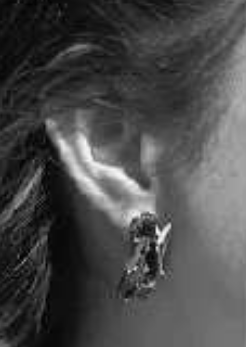
\includegraphics[width=.7\linewidth, height=5cm]{Imagenes/w1}
     \caption{Pendiente que mide la presión de la sangre}
     \label{fig:w1}
   \end{minipage}\hfill
   \begin {minipage}{0.48\textwidth}
     \centering
     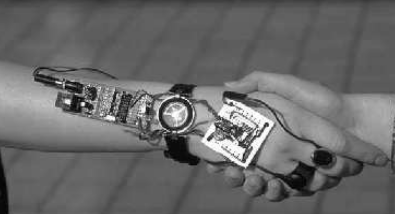
\includegraphics[width=.7\linewidth, height=5cm]{Imagenes/w2}
     \caption{Sensores y placa ajustados al brazo de una persona}
     \label{fig:w2}
   \end{minipage}
\end{figure}

\begin{figure}[]
   \begin{minipage}{0.48\textwidth}
     \centering
     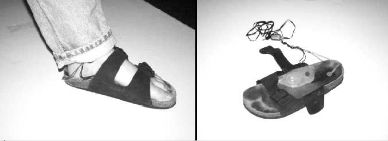
\includegraphics[width=.7\linewidth, height=5cm]{Imagenes/w3}
     \caption{Zapato utilizado para medir la conductancia de la piel}
     \label{fig:w3}
   \end{minipage}\hfill
   \begin {minipage}{0.48\textwidth}
     \centering
     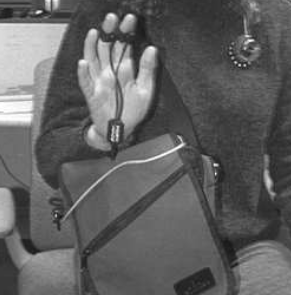
\includegraphics[width=.7\linewidth, height=5cm]{Imagenes/w4}
     \caption{Cámara digital, ordenador \textit{wearable} y sensores de la conductancia de la piel}
     \label{fig:w4}
   \end{minipage}
\end{figure}

\begin{figure}[]
   \begin{minipage}{0.48\textwidth}
     \centering
     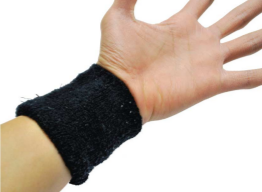
\includegraphics[width=.7\linewidth, height=5cm]{Imagenes/w5}
     \caption{Muñequera que mide la actividad electrodérmica de la piel}
     \label{fig:w5}
   \end{minipage}\hfill
   \begin {minipage}{0.48\textwidth}
     \centering
     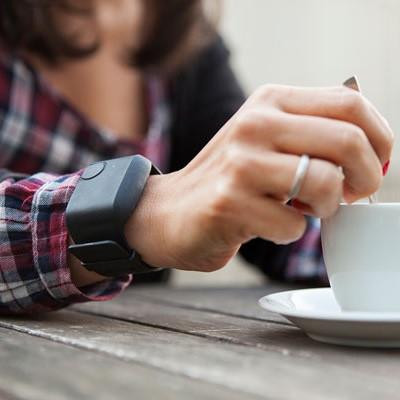
\includegraphics[width=.7\linewidth, height=5cm]{Imagenes/w6}
     \caption{Wristband de Empatica E4 que mide numerosas señales fisiológicas}
     \label{fig:w6}
   \end{minipage}
\end{figure}

\begin{figure}[]
   \begin{minipage}{0.48\textwidth}
     \centering
     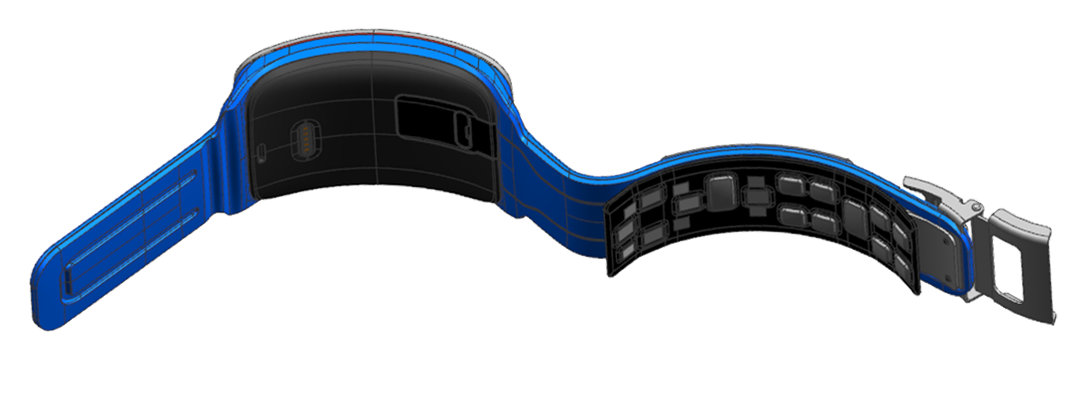
\includegraphics[width=.7\linewidth, height=5cm]{Imagenes/w7}
    \caption{Samsung Simband que mide numerosas señales fisiológicas}
     \label{fig:w7}
   \end{minipage}\hfill
   \begin {minipage}{0.48\textwidth}
     \centering
     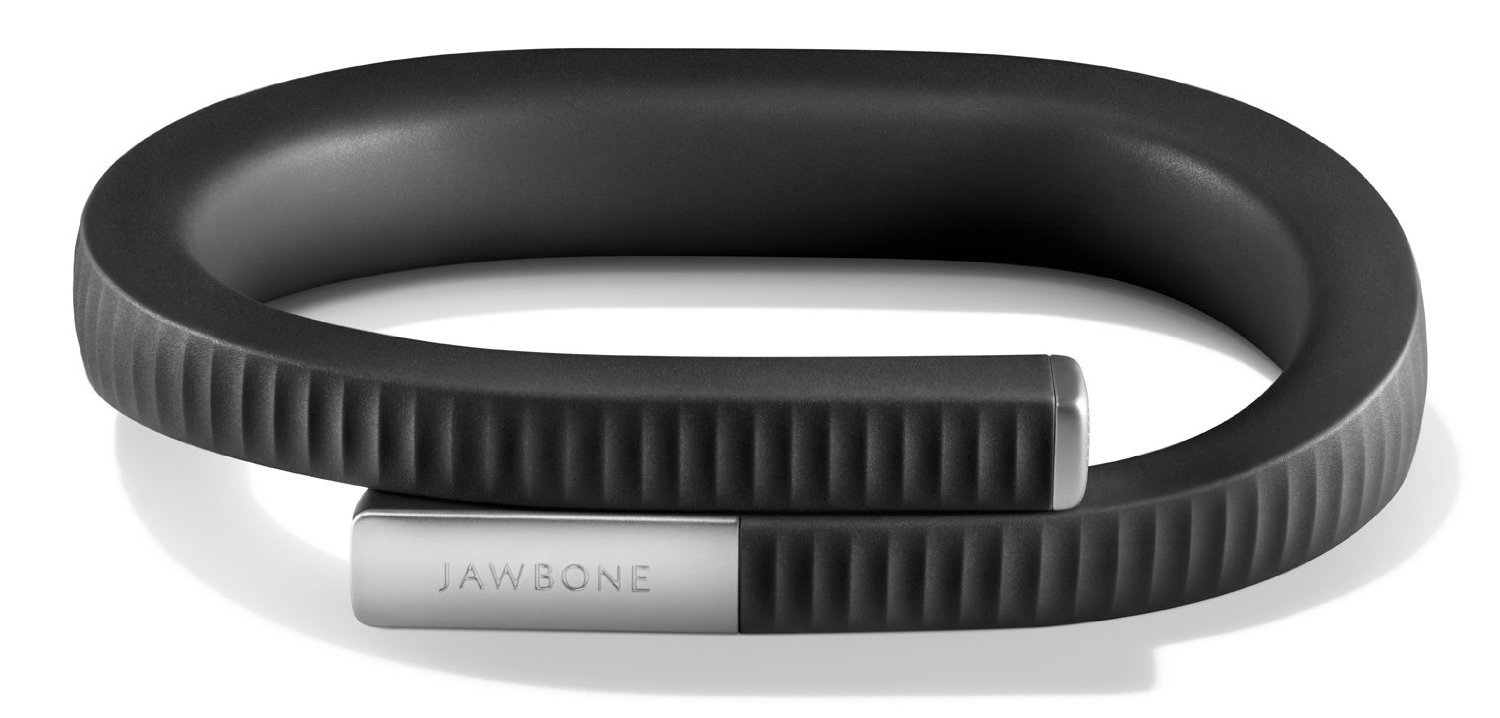
\includegraphics[width=.7\linewidth, height=5cm]{Imagenes/w8}
     \caption{Jawbone UP 24 que se utiliza para mejorar el rendimiento deportivo}
     \label{fig:w8}
   \end{minipage}
\end{figure}

%-------------------------------------------------------------------

\subsubsection{Pulseras inteligentes}
\label{subsubsec:pulserasInteligentes}
\paragraph{}
Actualmente existe una gran cantidad de pulseras inteligentes enfocadas a personas que quieran mejorar su rendimiento deportivo así como diversos estudios que comparan su fiabilidad \citep{sushames2016validity} \citep{baroni2015fitbit} \citep{kooiman2015reliability}. En esta sección se ha optado sin embargo por no saturar los ejemplos de las pulseras inteligentes de este último tipo puesto que es un enfoque que se aleja bastante del desarrollo de este trabajo. A continuación, se van a describir las características principales de una serie de pulseras inteligentes que sirven para medir distintas variables fisiológicas:

\begin{itemize}
    \item Fitbit Flex (\citeyear{martinez2015wristband}).
    \begin{itemize}
        \item Señales sensorizadas: ACC, HR.
        \item Objetivo: monitorización del sueño y de la actividad física.
        \item Fiabilidad: en un estudio que medía la monitorización del sueño con 107 sujetos realizada a lo largo de 7 días, el 86\% de los dispositivos no reconoció el sueño en 4 de estos 7 días y el 35\% de los dispositivos fue incapaz de reconocer el sueño en los 7 días del experimento\citep{baroni2015fitbit}. Otro estudio que medía la fiabilidad del contador del pasos con 48 muestras constataba que su validez es moderada, pues llegaba a tener margenes de error en el conteo de pasos de en torno al 20\%\citep{sushames2016validity}. Sin embargo, en una versión posterior llamada Fitbit Zip, esta pulsera fue la que obtuvo el menor margen de error entre otras 9 pulseras inteligentes en lo que respecta al conteo de pasos\citep{kooiman2015reliability}.
        \item Precio: actualmente está descatalogado. En el 2015 su precio era de 81€. Sus versiones posteriores cuestan en su tienda oficial entre 60 y 200€.
    \end{itemize}

    \item Jawbone UP 24 (\citeyear{jawbone24}).
    \begin{itemize}
        \item Señales sensorizadas: no especificadas en su documentación. A través de su API no es posible acceder a los datos sensorizados. Únicamente se pueden obtener datos procesados como los momentos en los que el usuario ha estado durmiendo.
        \item Objetivo: monitoreo de actividad física, del sueño y entrenador personal que aconseja al usuario para que tome decisiones saludables.
        \item Fiabilidad: según Tudor-Locke, los monitores de actividad no deberían sobrepasar un error del 1\% respecto a las mediciones del estándar de oro (en este caso respecto a las mediciones de pasos de Optogait\citeyear{optogait} en el laboratorio) para una prueba de conteo de pasos en una cinta mecánica a 4.8km/h para ser considerados fiables \citep{tudor2011many}. Siguiendo este mismo estándar, Jawbone UP es fiable según el estudio de Kooiman (\citeyear{kooiman2015reliability}).
        \item Precio: 75€.
    \end{itemize}

    \item Samsung Simband (\citeyear{simband}).
    \begin{itemize}
        \item Señales sensorizadas: ECG, PPG, ACC, ICG, EDA, SKT.
        \item Objetivo: monitoreo de señales fisiológicas.
        \item Fiabilidad: no se ha encontrado ningún estudio independiente que evalúe este producto.
        \item Precio: actualmente (2018) es gratuita para los investigadores tras rellenar una solicitud. Sin embargo, estas no siempre son aceptadas.
    \end{itemize}

    \item Empatica E4 (\citeyear{garbarino2014empatica}).
    \begin{itemize}
        \item Señales sensorizadas: EDA, PPG, SKT, HR, ACC.
        \item Objetivo: monitoreo de señales fisiológicas.
        \item Fiabilidad: a partir de un experimento con 7 sujetos, se exportó las señales ECG y PPG tanto con esta pulsera como con el estándar de oro con el que se comparó su fiabilidad, SEER Light Extend Recorder de General Electric. Las señales obtenidas fueron luego evaluadas por expertos y estudiantes de biomedicina, que evaluaban si la señal que observaban era real o no. El resultado obtenido fue que en el 85\% de los casos, ambos aparatos devolvieron datos con calidad similar, obteniendo datos de mejor calidad con el sensor de General Electric en un 5\% de los casos \citep{mccarthy2016validation}.
        \item Precio: 1372€.
    \end{itemize}

    \item Dispositivo: MoodMetric (\citeyear{moodmetric}).
    \begin{itemize}
        \item Señales sensorizadas: EDA.
        \item Objetivo: monitoreo de señales fisiológicas.
        \item Fiabilidad: en un estudio del instituto finés de ocupación para la salud con 24 voluntarios de entre 19 a 31 años se compararon las señales sensorizadas de EDA del prototipo de este anillo con un aparato de laboratorio para medir esa misma señal fisiológica, SA9309M. El resultado obtenido fue de una similaridad de la señal entre ambos dispositivos en un 83 y 16,4\% de los casos, concluyendo que dicho protitipo \textit{es un dispositivo prometedor para estudios ecológicamente válidos} \citep{torniainen2015feasibility}.
        \item Precio: 1.372€.
    \end{itemize}

\end{itemize}

\subsubsection{Comparativa de pulseras inteligentes}
\label{subsubsec:comparativaPulseras}
\paragraph{}
En la tabla~\ref{tab:accesoriosComparativa} se muestra una comparativa de los accesorios inteligentes citados en la sección anterior en base a la caracterización fisiológica de la ira descrita en la sección~\ref{subsubsec:fisioIra}. Como se puede ver en la tabla~\ref{tab:accesoriosComparativa}, se han descartado cinco de las trece características de la ira puesto que estas no se pueden medir con pulseras o anillos inteligentes al hacer referencia a variaciones de partes del cuerpo que no incluyen a los dedos de las manos o las muñecas (es el caso de la temperatura periférica facial) o ser referencias a sensaciones subjetivas que no se pueden discretizar de manera directa mediante pulseras o anillos inteligentes (es el caso de la sensación de desmayo, los sudores fríos, dolor de estómago y náuseas).

\paragraph{}
Como se puede ver en la tabla~\ref{tab:accesoriosComparativa}, los dos accesorios inteligentes que miden más señales fisiológicas de la ira son Samsung Simband y Empatica E4. Existen otra serie de elementos que pueden ayudar a seleccionar la mejor de las opciones entre ambas, como puede ser el precio, el tamaño y actividad de las comunidades de desarrolladores que utilizan estos productos o la versatilidad de sus \ac{SDK}. [TODO: según la solución que finalmente se elija, completar este párrafo de una u otra manera]

\paragraph{}
Respecto a las otras opciones comparadas, Jawbone UP 24 no está diseñada para ser utilizada por investigadores pues ni siquiera provee la caracterización de los sensores utilizados (de ahí que no haya sido posible cumplimentar la tabla para este accesorio inteligente). Fitbit Flex puede sensorizar la tasa cardíaca y los temblores a partir de su acelerómetro. Este accesorio, sin embargo, incluso en el caso de que pudiese sensorizar más información que el resto de accesorios debería ser descartada por sus grandes fallas de medición, tal y como se comentó en la sección~\ref{subsubsec:pulserasInteligentes}. Por último, el anillo de Moodmetric tiene el problema de ser excesivamente limitado, pues sólo es capaz de medir la actividad electrodérmica de la piel.

[TODO: según la solución que finalmente se elija, completar con un párrafo adicional de una u otra manera]


\begin{landscape}
\thispagestyle{plain}
\begin{table}[]
\centering
\caption{Comparativa de accesorios inteligentes para la medición de la ira}
\label{tab:accesoriosComparativa}
\begin{tabular}{|c|c|c|c|c|c|c|c|c|}
\hline
                                            & \textbf{\begin{tabular}[c]{@{}c@{}}Presión\\ arterial\end{tabular}} & \textbf{\begin{tabular}[c]{@{}c@{}}Tasa\\ cardíaca\end{tabular}} & \textbf{\begin{tabular}[c]{@{}c@{}}Tasa\\ respiratoria\end{tabular}} & \textbf{Temblores} & \textbf{\begin{tabular}[c]{@{}c@{}}Enrojecimiento\\ de la piel\end{tabular}} & \textbf{\begin{tabular}[c]{@{}c@{}}Tensión\\ muscular\end{tabular}} & \textbf{\begin{tabular}[c]{@{}c@{}}Sudor en\\ las manos\end{tabular}} & \textbf{\begin{tabular}[c]{@{}c@{}}Coductividad\\ de la piel\end{tabular}} \\ \hline
\textbf{Fitbit Flex}                                               & \xmark                                                                  & \cmark                                                               & \xmark                                                                   & \cmark                 & \xmark                                                                           & \xmark                                                                  & \xmark                                                                    & \xmark                                                                         \\ \hline
\textbf{Empatia E4}                                                & \cmark                                                                  & \cmark                                                               & \xmark                                                                   & \cmark                 & \xmark                                                                           & \xmark                                                                  & \xmark                                                                    & \cmark                                                                         \\ \hline
\textbf{MoodMetric}                                                & \xmark                                                                  & \xmark                                                               & \xmark                                                                   & \xmark                 & \xmark                                                                           & \xmark                                                                  & \xmark                                                                    & \cmark                                                                         \\ \hline
\end{tabular}
\end{table}
\end{landscape}

%-------------------------------------------------------------------

\section{Código deontológico}
\label{section:codDeonto}

\subparagraph{}
Puesto que en este proyecto se va a realizar una evaluación con seres humanos, es necesario conocer el código deontológico utilizado en psicología con el fin de evitar malas prácticas. Para este proyecto, se ha seguido el código deontológico utilizado por el Consejo General de Colegios Oficiales de Psicólogos de España en su versión aprobada el 6 de marzo de 2010 (a pesar de realizar este trabajo como informático y por tanto no estar regido por dicho código deontológico, se considera imprescindible asumir de propia iniciativa dicho código deontológico). Los principales postulados que afectan directamente a la investigación de este proyecto son los siguientes:
\begin{itemize}
    \item Finalidad humana y social de la psicología.
    \item Respeto a la persona y protección de los derechos humanos.
    \item No realización de prácticas que atenten contra la libertad e integridad psíquica y física de las personas.
    \item Utilización cautelar del lenguaje con el fin de evitar etiquetas devaluadoras y discriminatorias.
    \item Asegurar la libertad de los sujetos a la hora de formar parte del experimento.
    \item Respeto de la intimidad de los sujetos conjugada a través de la no divulgación de los datos obtenidos sin que estos hayan sido previamente anonimizados.
\end{itemize}